\documentclass[12pt,letterpaperpaper,]{book}
\usepackage{lmodern}
\usepackage{amssymb,amsmath}
\usepackage{ifxetex,ifluatex}
\usepackage{fixltx2e} % provides \textsubscript
\ifnum 0\ifxetex 1\fi\ifluatex 1\fi=0 % if pdftex
  \usepackage[T1]{fontenc}
  \usepackage[utf8]{inputenc}
\else % if luatex or xelatex
  \ifxetex
    \usepackage{mathspec}
  \else
    \usepackage{fontspec}
  \fi
  \defaultfontfeatures{Ligatures=TeX,Scale=MatchLowercase}
    \setmonofont[Mapping=tex-ansi,Scale=0.8]{Source Code Pro}
\fi
% use upquote if available, for straight quotes in verbatim environments
\IfFileExists{upquote.sty}{\usepackage{upquote}}{}
% use microtype if available
\IfFileExists{microtype.sty}{%
\usepackage{microtype}
\UseMicrotypeSet[protrusion]{basicmath} % disable protrusion for tt fonts
}{}
\usepackage[margin=1in]{geometry}
\usepackage{hyperref}
\hypersetup{unicode=true,
            pdftitle={DRAFT Dissertation Prospectus},
            pdfauthor={Danton Noriega},
            pdfborder={0 0 0},
            breaklinks=true}
\urlstyle{same}  % don't use monospace font for urls
\usepackage{natbib}
\bibliographystyle{apalike}
\usepackage{longtable,booktabs}
\usepackage{graphicx,grffile}
\makeatletter
\def\maxwidth{\ifdim\Gin@nat@width>\linewidth\linewidth\else\Gin@nat@width\fi}
\def\maxheight{\ifdim\Gin@nat@height>\textheight\textheight\else\Gin@nat@height\fi}
\makeatother
% Scale images if necessary, so that they will not overflow the page
% margins by default, and it is still possible to overwrite the defaults
% using explicit options in \includegraphics[width, height, ...]{}
\setkeys{Gin}{width=\maxwidth,height=\maxheight,keepaspectratio}
\IfFileExists{parskip.sty}{%
\usepackage{parskip}
}{% else
\setlength{\parindent}{0pt}
\setlength{\parskip}{6pt plus 2pt minus 1pt}
}
\setlength{\emergencystretch}{3em}  % prevent overfull lines
\providecommand{\tightlist}{%
  \setlength{\itemsep}{0pt}\setlength{\parskip}{0pt}}
\setcounter{secnumdepth}{5}
% Redefines (sub)paragraphs to behave more like sections
\ifx\paragraph\undefined\else
\let\oldparagraph\paragraph
\renewcommand{\paragraph}[1]{\oldparagraph{#1}\mbox{}}
\fi
\ifx\subparagraph\undefined\else
\let\oldsubparagraph\subparagraph
\renewcommand{\subparagraph}[1]{\oldsubparagraph{#1}\mbox{}}
\fi
\usepackage{booktabs}
\usepackage{lscape}
\usepackage{longtable}
\usepackage{bm}
\usepackage{isomath}
\usepackage{setspace}
% \doublespacing
\usepackage[bf,singlelinecheck=off]{caption}
\newcommand{\matr}[1]{\mathbf{#1}}
\newcommand{\blandscape}{\begin{landscape}}
\newcommand{\elandscape}{\end{landscape}}

\setromanfont[Mapping=tex-text]{Minion Pro}
\setsansfont[Mapping=tex-text]{Source Sans Pro}
\setmonofont[Mapping=tex-text,Scale=0.8]{Source Code Pro}

\usepackage{framed,color}
\definecolor{shadecolor}{RGB}{248,248,248}

\renewcommand{\textfraction}{0.05}
\renewcommand{\topfraction}{0.8}
\renewcommand{\bottomfraction}{0.8}
\renewcommand{\floatpagefraction}{0.75}

% \renewenvironment{quote}{\begin{VF}}{\end{VF}}
\let\oldhref\href
\renewcommand{\href}[2]{#2\footnote{\url{#1}}}

\ifxetex
  \usepackage{letltxmacro}
  \setlength{\XeTeXLinkMargin}{1pt}
  \LetLtxMacro\SavedIncludeGraphics\includegraphics
  \def\includegraphics#1#{% #1 catches optional stuff (star/opt. arg.)
    \IncludeGraphicsAux{#1}%
  }%
  \newcommand*{\IncludeGraphicsAux}[2]{%
    \XeTeXLinkBox{%
      \SavedIncludeGraphics#1{#2}%
    }%
  }%
\fi

\makeatletter
\newenvironment{kframe}{%
\medskip{}
\setlength{\fboxsep}{.8em}
 \def\at@end@of@kframe{}%
 \ifinner\ifhmode%
  \def\at@end@of@kframe{\end{minipage}}%
  \begin{minipage}{\columnwidth}%
 \fi\fi%
 \def\FrameCommand##1{\hskip\@totalleftmargin \hskip-\fboxsep
 \colorbox{shadecolor}{##1}\hskip-\fboxsep
     % There is no \\@totalrightmargin, so:
     \hskip-\linewidth \hskip-\@totalleftmargin \hskip\columnwidth}%
 \MakeFramed {\advance\hsize-\width
   \@totalleftmargin\z@ \linewidth\hsize
   \@setminipage}}%
 {\par\unskip\endMakeFramed%
 \at@end@of@kframe}
\makeatother

\newenvironment{rmdblock}[1]
  {
  \begin{itemize}
  \renewcommand{\labelitemi}{
    \raisebox{-.7\height}[0pt][0pt]{
      {\setkeys{Gin}{width=3em,keepaspectratio}\includegraphics{images/#1}}
    }
  }
  \setlength{\fboxsep}{1em}
  \begin{kframe}
  \item
  }
  {
  \end{kframe}
  \end{itemize}
  }
\newenvironment{rmdnote}
  {\begin{rmdblock}{note}}
  {\end{rmdblock}}
\newenvironment{rmdcaution}
  {\begin{rmdblock}{caution}}
  {\end{rmdblock}}
\newenvironment{rmdimportant}
  {\begin{rmdblock}{important}}
  {\end{rmdblock}}
\newenvironment{rmdtip}
  {\begin{rmdblock}{tip}}
  {\end{rmdblock}}
\newenvironment{rmdwarning}
  {\begin{rmdblock}{warning}}
  {\end{rmdblock}}

\usepackage{makeidx}
\makeindex

\urlstyle{tt}

\usepackage{amsthm}
\makeatletter
\def\thm@space@setup{%
  \thm@preskip=8pt plus 2pt minus 4pt
  \thm@postskip=\thm@preskip
}
\makeatother

\title{DRAFT Dissertation Prospectus}
\author{Danton Noriega}
\date{November 26, 2016}

\begin{document}
\maketitle

\setlength{\abovedisplayskip}{-5pt}
\setlength{\abovedisplayshortskip}{-5pt}
\mainmatter

{
\setcounter{tocdepth}{2}
\tableofcontents
}
\chapter{An Evaluation of the Double Up Food Bucks
program}\label{chapter-1}

\section*{Introduction}\label{intro-1}
\addcontentsline{toc}{section}{Introduction}

Chronic conditions like obesity, heart disease, and other metabolic risk
factors (stroke, type II diabetes, etc.) are estimated to cost the US
health care system between 200 to 400 billion dollars annually
\citep{cawley_medical_2012, chatterjee_checkup_2014}. More importantly,
these diseases account for hundreds of thousands of deaths each year.
Heart disease alone is the leading cause of death for all persons in the
US, with stroke fifth and diabetes seventh
\citep{national_center_for_health_statistics_health_2015}. Diet is
closely linked to these conditions, particularly obesity and
cardiovascular disease. There is strong evidence that a diet high in (1)
vegetables, fruits, nuts, unsaturated oils, fish, and poultry, but low
in (2) red and processed meat and sugar-sweetened foods and drinks,
helps lower body weight, blood pressure, and the risk of cardiovascular
disease
\citep{mente_systematic_2009, nutrition_evidence_library_series_2014}.
Improving the diet of Americans has therefore become an increasing
priority for the United States, especially for struggling families that
participate in the Supplemental Nutrition Assistance (SNAP) program.

SNAP is a federal aid program administered by the Food and Nutrition
Service (FNS), an agency of the U.S. Department of Agriculture (USDA).
At 74 billion dollars in FY2015 with roughly 45.8 million participants,
it is the largest food assistance program in the US
\citep{usda_fns_supplemental_2016}. To be eligible for SNAP, a household
must be sufficiently budget constrained that hunger is considered likely
without assistance. Eligibility is a function of countable resources,
vehicle ownership and value, household size, gross or net monthly
income, household composition, and meeting certain work
requirements.\footnote{For more details, visit
  \url{http://www.fns.usda.gov/snap/eligibility}} Some eligibility
requirements vary by state, but in general, a family with less than
\$2000 in countable resources, where the adults work at least part-time
earning a gross (net) monthly income at or below 130\% (100\%) of the
federal poverty line, is eligible to receive SNAP benefits. Aside from a
few restrictions---no alcohol, tobacco, non-food items, read-to-eat
meals, or hot foods---households can use SNAP benefits to purchase any
foods that will be prepared and consumed at home. Unfortunately, the
purchasing patterns of the average SNAP household are not conducive to a
healthy diet.

Research on the dietary patterns of households receiving SNAP benefits
has found that they are significantly \emph{less} likely to meet USDA
dietary guidelines than the average US household and much \emph{more}
likely to consume unhealthy foods
\citep{andreyeva_dietary_2015, nguyen_supplemental_2015, wolfson_fruit_2015}.
A smaller set of research has found that SNAP households, at best,
consume same amount of unhealthy foods (e.g.~sugar-sweetened beverages,
baked goods, snacks, candy, etc) compared to SNAP-ineligible households
\citep{todd_caloric_2014, hoynes_snap_2015}. In other words, SNAP
households consume foods that are less healthy or about the same as
SNAP-ineligible households. This is a concerning result given that most
US households, regardless of income, already purchase and consume far
too much meat and foods rich in sugars and fats, and far too few fruits,
vegetables and whole grains
\citep{usda_scientific_2015, frazao_high_1999}. However, the purpose of
SNAP is to keep struggling families from going hungry, not to ensure
they consume the best possible diet. SNAP is designed to act like cash,
helping families access more food than they could otherwise do so
without assistance \citep{hoynes_snap_2015}. It is therefore not a
failing of the SNAP program if benefits are used to purchase unhealthy
foods.

The SNAP program could be change such that it could continue satisfying
its role as an anti-hunger program while simultaneously encouraging
healthier purchases. \citet{blumenthal_strategies_2014} and
\citet{leung_qualitative_2013} both surveyed a field of stakeholders and
policy experts in the SNAP program about what they would do to improve
the dietary quality of purchases. In both studies, restricting the
purchase of unhealthy foods (e.g.~sugar-sweetened beverages) and
promoting healthy purchases through monetary incentives were the two
most popular improvements (i.e.~ranked the highest or most often
suggested).\footnote{It should be mentioned that there were other, less
  popular recommendations, such as modifying how SNAP benefits are
  distributed and improving nutrition education. For more details, see
  \citet{blumenthal_strategies_2014} and \citet{leung_qualitative_2013}}.

One common suggestion is to restrict the SNAP program to the same set of
eligible foods as the Woman, Infants, and Children (WIC) program
\citep{dinour_food_2007}. The WIC program provides food vouchers which
limit households to a select group of food products. These food products
are specifically selected to ensure women and their children receive
nutritious, healthy foods. In other words, the WIC program, by design,
places restrictions on food choices by defining a list of
\emph{eligible} items, as opposed to the SNAP program, which defines a
list of \emph{ineligible} items. Another common, and simpler, suggestion
is to expand the existing list of ineligible items (e.g.~alcohol) with
products that are unambiguously lacking in nutrition and easy to
identify, like soda or candy. New York City, for example, attempted to
ban the purchase of sugar-sweetened beverages, and the state of Maine
attempted to restrict the purchase of sodas, candy, and any other
taxable food items \citep{gundersen_snap_2015}. Both restrictions were
overturned by the USDA.

There are problems with ``improving'' the SNAP program by implementing
even greater purchasing restrictions. First, there is no reason to
believe that such a restriction would work. The restriction assumes
that, under WIC-like requirements, households will substitute healthy
foods for unhealthy foods when using SNAP benefits. What would most
likely happen is that households would shift to purchasing unhealthy
foods with cash. Second, such restrictions would likely lead to a drop
in SNAP participation \citep{gundersen_snap_2015}. Restricting choice is
a paternalistic policy that would further stigmatize SNAP participation.
It would give the impression that SNAP beneficiaries are assumed to have
worse diets and that they cannot be trusted to make healthy food
purchases. Participation would also drop due to increased transactions
costs of purchasing items with SNAP. Not all stores would clearly mark
which items were SNAP eligible nor should participants be expected to
remember. The result would be longer, more frustrating shopping trips.
Lastly, it is important to remember that for many SNAP recipients,
freedom of choice is what makes the SNAP program popular and easy to use
\citep{edin_snap_2013}.

The most popular ``improvement'' was providing a monetary incentive to
SNAP participants for purchasing healthy foods
\citep{blumenthal_strategies_2014, leung_qualitative_2013}. Monetary (or
financial) incentives, in this context, tend to be a rebate or voucher
awarded to SNAP households for using their benefits to buy certain
healthful foods, generally mineral-rich and nutrient-dense fruits and
vegetables (i.e.~leafy greens but not white potatoes). These monetary
incentives for buying ``targeted'' fruits and vegetables (aka TFVs) are
exclusive to SNAP participants. Much like a grocery stores loyalty card
or a student ID card, retailers can ``discriminate on price'' (aka
``target the incentive'') using SNAP Electronic Benefit Transfer (EBT)
cards to identifying eligible participants. Monetary incentives in the
food retail environment are popular for two main reason. First, the
framing of the ``improvement'' is positive. Instead of ``punishing''
SNAP participants through paternal restriction or disincentives (not
covered), monetary incentives reward participants for healthy shopping
behavior \citep{gundersen_snap_2015}. Retailers also prefer the positive
framing of monetary incentives. For the moment, monetary incentives
programs for SNAP participants are not wide spread. Therefore, taking up
an incentive program, assuming the cost of implementation isn't too
expensive, creates an opportunity for retailers to differentiate
themselves from their competitors \citep{hartmann_corporate_2011}. The
second reason is a strong theoretical framework established by
neoclassical economics supporting incentives as an effective mechanism
for changing human behavior. In practice, however, incentives have had
mixed results, but there is building evidence that incentives may work
in the food retail space.

How, why, and to what effect incentives may encourage SNAP participants
to purchase more targeted fruits and vegetables will be discussed in
detail below, and is the motivating question behind this paper.

\subsection*{Financial Incentives to Encourage Healthy Food
Purchases}\label{financial-incentives-to-encourage-healthy-food-purchases}
\addcontentsline{toc}{subsection}{Financial Incentives to Encourage
Healthy Food Purchases}

Encouraging healthy behavior through financial incentives has a long
history. Results are mixed. For example, financial incentives have been
shown to help individuals commit to regular exercise, improve dieting,
increase weight loss, and to quit smoking, but the intended effect of
the financial incentives were often only short-term (see
\citet{gneezy_when_2011} and \citet{cawley_economy_2015} for an
overview). \citet{gneezy_when_2011} also explain, through a review of
the literature, that depending on the context and design, incentives can
backfire, producing an effect known as ``crowd out''. Crowd out occurs
when an incentive displaces the intrinsic reward of a behavior
(originally defined for ``prosocial'' behavior, like volunteering or
giving blood; see \citet{benabou_incentives_2006}). The behavior then
becomes dependent on the extrinsic reward. As a result, having shifted
from being intrinsically rewarding to extrinsically rewarding, the
positive behavior continues only as long as the monetary incentive is
provided. More significantly, the intrinsic reward of the behavior does
not return once it has been ``crowded out''. Therefore, the long-term
effect of a monetary incentive can be negative, despite showing positive
effects in the short-term. That said, incentives can produce successful
long-term results if they are instead used as a mechanism to build good
habits. This requires that the incentives be salient and produce
immediate feedback without neglecting behavioral findings such as loss
aversion and mental accounting \citep{john_financial_2011}.

Given the research on incentives, it is reasonable to assume that a
monetary incentive for SNAP participants to purchase healthy foods, like
fruits and vegetables, may fail or even backfire. Should the act of
purchasing healthy foods be intrinsically rewarding to SNAP shoppers,
introducing an incentive may produce a ``crowd out'' effect. However,
recent field experiments find that incentives can establish healthy food
choice as a habit, possibly overriding any crowd out. Daily incentives
encourage children to make healthier food choices in school lunchrooms,
who in turn develop positive, long-term food habits
\citep{loewenstein_habit_2016, list_behavioralist_2015, belot_incentives_2014}.
Outside of the school lunchroom environment,
\citet{list_incentives_2015} found that similar habit formation is
possible with incentives in a more traditional food retail environment.
In their experiment, \citet{list_incentives_2015} provided an incentive
to 222 shoppers (\$1) to use their rewards cards, but then randomly
assigned each participant to the control group to one of three
interventions: \emph{information}, \emph{incentive}, or
\emph{combination}. The \emph{information} treatment was a flyer with
tips on how to prepare fruit and vegetable dishes as well as the health
benefits of eating more fruits and veggies. The \emph{incentive} was an
additional dollar for every 5 cups of targeted fruits and vegetables
(TFVs) purchased. The \emph{combination} treatment group included both.
The intervention lasted for 5 months but each group continued to be
observed for roughly 6 weeks months after. The \emph{information}
intervention had no effect, but the \emph{incentive} and
\emph{combination} interventions on average doubled their purchase of
fruits and vegetables in comparison to the control group. Most
promisingly, the gap persisted with minimal shrinkage for 6 weeks
following the end of the intervention. However, there was no follow up
after the 6-week post-intervention period. It is therefore possible the
gap closed over multiple months (as opposed to multiple weeks).

The design, food environment, and target of the incentive in each of
these experiments is important. First, the incentive in these
experiments is designed to be salient and immediate. In the school
lunchroom experiments, the children are aware of the incentive and
receive the reward (e.g.~a small token) immediately after selecting the
healthy food item. Likewise, the shoppers received their additional \$1
reward for every 5 cups of TFVs at checkout. One distinction between the
designs is frequency. The children are exposed to the incentive every
school day in the lunchroom experiments. The shoppers, on the other
hand, were exposed as frequently or as infrequently as they chose. This
distinction is important, as the latter better reflects the experience
of shoppers using the SNAP benefits. Second, the food environment is
important because it determines what choices are available. The children
have a finite set of options in the school lunchroom and they also have
no outside option (besides not eating lunch). The children optimize on a
relatively small set of choices and, for the duration of the
intervention, the incentive always existed. Food retail environments are
drastically different. There are numerous competing food choices and
generally other outside options.\footnote{It should be noted that this
  is not always the case. In \citet{list_incentives_2015}, for example,
  the store that was selected for the experiment was one of the few
  places local shoppers could find fresh produce. The store itself was
  located in one of Chicago's poorer neighborhoods.} It is substantially
more difficult for the shopper to optimize over such a large set of
choices. Last, and most obviously, one set of studies targets children,
the other adults. A priori, we would expect a monetary incentive to
affect children differently than adults. The fact that habit formation
through incentives appears possible for both target groups is promising.

Research where SNAP participants are the target group is nascent. The
USDA's Food and Nutrition Services (FNS) ran the first large scale
randomized control trial investigating the impact of a financial
incentive for targeted fruits and vegetables in 2011. The experiment was
called the Healthy Incentives Pilot (HIP). HIP is the precursor to every
incentive program currently being funding by the USDA. It also provides
the data for the few papers recently published on incentives for SNAP
participants.

\subsection*{The Healthy Incentives
Pilot}\label{the-healthy-incentives-pilot}
\addcontentsline{toc}{subsection}{The Healthy Incentives Pilot}

A brief overview of the Healthy Incentives Pilot is necessary to provide
context to, and contrast with, more recent financial incentive programs.

The UDSA's Food and Nutrition Services designed the Healthy Incentives
Pilot. The pilot was funded by the Food, Conservation, and Energy Act of
2008 to test whether financial incentives would increase consumption of
targeted fruits and vegetables (TFVs). SNAP participants were the target
group.

HIP was designed as a large scale randomized control trial (RCT). FNS
partnered with the Massachusetts Department of Transitional Assistance
to implement HIP. The pilot lasted from early 2011 to the end of 2012.
The population included all 55,095 SNAP participants in Hampden County,
MA. Hampden County is the poorest county in Massachusetts and has the
highest rates of obesity and other diet-related chronic illness
(e.g.~type 2 diabetes).

Of the 55,095 SNAP participants, 7,500 were randomly assigned to the
treatment group. The remainder fell into the control group. The
treatment was a 30 cent (or 30\%) rebate on every dollar spent on TFVs.
The rebate was capped at \$60 per month. To receive the rebate, selected
SNAP participants had to use their EBT cards at participating retailers.
The rebate, which was returned to their EBT account, could then be used
on any food item. That is, the rebate could only be earned buying TFVs,
but could be redeemed buying any SNAP eligible food item. Most HIP
participants spent about \$12 a month on TFVs, earning an average of
\$3.65 per month in rebates---drastically lower than the \$60 per month
rebate cap.

The evaluation was conducted using 24-hour dietary recall surveys. A
total of 5,000 participants were selected to be surveyed, even split
between treatment and control (2,500 HIP, 2,500 non-HIP). The first
survey was conducted prior to the start of the pilot. This established a
baseline. The second survey occurred 4 to 6 months in to the pilot and
the third survey occurred 9 to 11 months in. (The variation, e.g.~4 to 6
months, was due to the treatment being implemented in 3 waves of 2500.)

The evaluation found that the 30\% rebate lead to about a 26\% increase
in consumption of TFVs. This was equivalent to about 0.24 cups of TFVs.
Roughly 60\% of the increase was due to increased vegetable consumption
and 40\% due to increased fruit consumption. The effect, in absolute
terms (0.24 cups), seems small. But a \(0.87\) price elasticity,
relative to other results in the literature, is quite high---\(0.7\) and
\(0.48\), on average, for fruits and vegetables, respectively
\citep{andreyeva_impact_2010}.

Despite some limitations and technical problems---underreporting on the
24-hour recall survey and system glitches early in the pilot (see pages
60 and 208-210 of \citet{bartlett_evaluation_2014})---HIP was considered
to be an overall success
\citep{klerman_short-run_2014, olsho_financial_2016}. It implemented on
of the largest, most complex RCTs to isolate how incentives can increase
household consumption of TFVs. It also provided a feasible model for
nationwide expansion (assuming cost reductions due to economies of
scale; see \citet{an_nationwide_2015}).

HIP also provides a framework for understanding how a financial
incentive, expanded dramatically in one geographic area, could improve
TFV consumption. But, as noted in the final HIP report, one of the most
prominent retailers in Hampden County chose not to participate (page 61,
\citet{bartlett_evaluation_2014}). Its third-party processor decided it
was too difficult and too costly to implement the financial incentive on
its point-of-sale technology. This strategic behavior by the retailer,
which had a significant presence in Hampden County, impacted where
participants could use the incentive.

Most financial incentive programs work at the local level, expanding
non-randomly. We should anticipate certain retailers (firms) to behave
strategically when participating in any of these incentive programs.
Likewise, we should anticipate voluntary (non-random) self-selection by
SNAP beneficiaries into these financial incentives programs. To this
end, more research is needed to understand the impact of incentive
programs under \emph{real-world} conditions. HIP provided evidence that
incentive programs can work, but barring state-wide or nation-wide
adoption of point-of-sale financial incentives, we should expect growth
to occur organically under non-experimental conditions.

An example of such a financial incentive program for SNAP participants
is the Double Up Food Bucks program (DUFB or Double Up). The non-random
expansion and impact of this financial incentives program will remain
the focus of this paper

\subsection*{The Double Up Food Bucks
Program}\label{the-double-up-food-bucks-program}
\addcontentsline{toc}{subsection}{The Double Up Food Bucks Program}

The success of HIP paved the way for the Food Insecurity Nutrition
Initiative (FINI), established by section 4208(b) of the Agricultural
Act of 2014 (aka 2014 Farm Bill). FINI---a 100-million-dollar
initiative---in turn piloted numerous non-profit financial incentive
programs aimed at improving the diets of SNAP participants.

Of specific interest is Double Up Food Bucks (DUFB or Double Up), an
incentives-based program funded by FINI. In 2009, the non-profit
organization Fair Food Network (FFN) launched the Double Up Food Bucks
program in Detroit, Michigan. The intention of the program was to get
more low-income families visiting and participating in local Detroit
farmer's markets. The mechanism for increasing participation was a
dollar-for-dollar match of locally grown fruit and vegetable purchases.
This subsidy was accessible only to low-income families receiving SNAP
benefits, who could exchange up to \$20 of their benefits for a wooden
token that could be used on up to \$40 worth of locally grown produce.

The DUFB program was considered successful given it had expanded to more
than 150 farmer's markets in 2014 from just 5 farmer's markets in 2009.
SNAP benefits have been used more than 200,000 times to purchase fresh
produce, with more than 10,000 first time SNAP customers visiting
farmer's markets in 2013 alone \citep{fair_food_network_double_2014}.
The program is considered by Fair Food Network to be a ``three-fold''
win given that the program helps local low-income families buy more
fresh produce, provides new customers for local farmer's, and stimulates
the local food economy. Relative to farmer's markets in other states,
DUFB did seem to be bringing in substantially more SNAP dollars (\$1.7
million in Michigan versus \$307,000 in Illinois, the second largest).

A 5.17 million dollar FINI grant was awarded to Fair Food Network to
help it pilot three adjustments to the Double Up Food Buck program
\citep{usda_nifa_usda_2015}. First, FFN needs to test DUFB as a
year-round program in select locations instead of the current seasonal
format. Second, shift away from the token system to providing DUFB
electronically at point-of-sale. Third, the DUFB needs to expand from
farmer's markets into other retail environments, like supermarkets and
grocery stores.

Successful expansion into supermarkets and grocery stores is critical.
Approximately 80\% of all SNAP benefits in 2015 were used in
supermarkets or super stores \citep{usda_fns_snap_2016}. Less than 1\%
percent of SNAP benefits were used at local farmer's markets. The amount
of SNAP benefits used in local farmer's markets has increased since
2009, but no where near the growth necessary to reach the type of stores
most frequented by low-income families. If localized financial incentive
programs like DUFB are going to be considered one of the USDA's many
tools to increase food access and combat obesity, then they must be
successfully implemented and scaled across supermarkets and grocery
stores. Most importantly, incentive programs like DUFB must prove they
are effective in changing purchasing habits within supermarket/grocery
store food environments.

\subsection*{Double Up Food Bucks vs the Healthy Incentives
Pilot}\label{double-up-food-bucks-vs-the-healthy-incentives-pilot}
\addcontentsline{toc}{subsection}{Double Up Food Bucks vs the Healthy
Incentives Pilot}

There are notable differences between DUFB and HIP that make the
evaluation of DUFB more difficult. In short, HIP was implemented as an
RCT. DUFB implementation is not. Let's explore in greater detail.

HIP had substantially more participating stores, all within the same
county (Hampden County, MA). DUFB has fewer participating stores, spread
across many different counties, and across many different grocery store
chains. Therefore, the probability of a SNAP shopper in Hampden County
having walked into a HIP participating store was much higher than a SNAP
shopper walking into any DUFB participating retailer.

The incentive delivery mechanisms also differ. First, all SNAP
beneficiaries who shop at a DUFB participating store receive the benefit
automatically. In other words, SNAP households that patron a store with
DUFB receive the incentive regardless of their intentions or awareness
of the DUFB incentive. Therefore, evaluating DUFB has the added
difficulty of identifying which shoppers are optimizing in response to
DUFB, as opposed to shopping normally. In contrast, SNAP households
assigned to the HIP treatment group were made aware of incentive and
were eligible to use it (even if they didn't quite understand how the
incentive program worked --- see \citet{bartlett_evaluation_2014}).
Households in the control group were not aware of the incentive and were
not eligible to use it. And because participants were assigned, HIP
evaluators could identify treated participants from control
participants.

Second, the DUFB financial incentive is substantially larger but more
restrictive. The DUFB incentive is a dollar-for-dollar match of locally
grown produce purchases capped at \$20 per day. The matched dollars are
accrued as points on a store loyalty card. Existing points are then
automatically redeemed as dollars on \emph{any} fresh produce purchases,
not just locally grown produce. In comparison, the HIP financial
incentive was a return of 30 cents per dollar spent on TFVs which could
be spent on \emph{any} food item. That is, the DUFB incentive doubled
the purchasing power of every dollars spent on TFVs \emph{only for more
TFVs}; the HIP incentive increased the purchasing power of every dollars
spent on TFVs by 30\% \emph{for any SNAP eligible food item}.

Finally, the experimental designed of HIP allowed researchers to form a
causal interpretation of their results; the average treatment effect is
the same as the average treatment effect on the treated. Any difference
in the purchase and consumption of TFV between the treatment and control
groups could therefore be attributed to the incentive. This is not the
case for DUFB. However, HIP implementation is the exception. How DUFB,
and similar financial incentive programs are implemented, is the norm.
The contribution of this paper will be evaluating and understanding the
impact of DUFB, given that DUFB and similar programs are implemented in
the ``real-world'' (non-experimental conditions)

\subsection*{Evaluating Double Up Food Bucks in Non-experimental
Conditions}\label{evaluating-double-up-food-bucks-in-non-experimental-conditions}
\addcontentsline{toc}{subsection}{Evaluating Double Up Food Bucks in
Non-experimental Conditions}

DUFB's expansion and implementation into supermarkets and grocery stores
did not follow an experimental design. Fair Food Network searched for
local partners in the Detroit area willing to participate in DUFB. Not
all grocery stores, especially the smaller independent stores, had the
capacity to implement the point-of-sale technology necessary for the
incentive---even if FFN offered to help cover the upgrade costs. The
result is a self-selected group of stores participating in DUFB. This,
in some ways, parallels what occurred in HIP, where one of the largest
retailers decided integrating their point-of-sale systems to include the
incentive was too expensive. This type of strategic firm behavior is
important to consider, even if complicates the evaluation of an
incentive program like DUFB.

In the real world, stores seek to maximize profits and will opt to
participate only if they expect to profit. Similarly, individuals will
self-select into participating; participation is optional and more
likely to occur with well-informed and motivated SNAP shoppers.
Selection, in this case, is a feature, not a flaw, of such incentive
programs when implemented by non-profits or policy makers. The evidence,
thanks to HIP, exists that incentives can lead to an increase in
consumption. The goal of this paper is therefore to accurately measure
the effect of the DUFB on TFV purchases while taking the selection into
account. That effect can then be extrapolated forward, albeit weakly,
using the results of HIP, to measure changes in consumption.

Fair Food Network started testing and gathering data from grocery stores
implementing DUFB in 2014. One of FFN's largest partners, a Michigan
grocery retail and distribution company, piloted the program in 2 of its
stores in 2014. The company has since expanded to 5 stores in 2015 and
then to 17 of 62 stores in 2016. Rapid scaling was possible due to the
point-of-sale technology used by the company to implement DUFB across
its stores. It provides, to date, the best case study of a firm
strategically scaling DUFB across numerous grocery stores that span
different geographic areas and populations.

All transaction data from 2014 - 2016 will be provided for every store
that has, at any point, participated in DUFB. These data are complete
(i.e.~no records have been removed) and at the item level. A complete
set of data will also be provided from another 15 stores where DUFB was
not implemented.

Currently, no research exists evaluating DUFB, or similar incentive
programs, using a complete set of store transaction data. HIP, for
example, only had transactions records for SNAP EBT cards. Transactions,
should a different tender be used by the same individual, could not be
observed. Therefore, these data provide an unprecedented opportunity to
analyze how the DUFB financial incentive performs under real-world
conditions. This paper will be, to the best of my knowledge, the first
to perform an evaluation of a financial incentive, targeted at SNAP
participants, using a complete set of data, from multiple stores, across
multiple years, and collected under non-experimental conditions.

\section*{Data}\label{data-1}
\addcontentsline{toc}{section}{Data}

These data come from a large grocery distributor and retailer serving
multiple grocery chains. Three years of data will be made available,
2014 through 2016. To my understanding, this includes months where the
DUFB incentive is active (Aug 1 to Dec 31) and inactive (Jan 1 to July
31) across all stores. These data are transaction level data and will
include (at least) store number, register, transaction ID, date and time
of purchase, payment type, item, dollars, and quantity.

Double Up implementation was considered for a single grocery chain. The
chain has more than 60 stores, 17 of which were selected as
``treatment'' stores (with Double Up). Of the remaining stores, data is
being made available from an addition 15 to serve as ``controls''. The
quotes here signify that these terms will be used as shorthand, but the
terminology is somewhat misleading. The use of ``treatment'' and
``control'' could lead one to think store assignment was random. It was
not.

{[}MISSING real specific details about the data e.g.~total transactions
observed etc.{]}

\textbf{Data Not Linked to Individuals}

One important variable that will not be made available is a variable for
loyalty card numbers. The company's use of loyalty cards across its many
chains was an exciting prospect. Previous transaction data from smaller
independent grocery chains had no way linking purchases to a single
unique identifier over time because these smaller chains did not have
advanced point-of-sale systems.

In earlier conversations with the company, it was understood that
loyalty cards would be made available. However, months into working with
the company, I was informed that this was no longer possible. Per the
company's legal department, the company cannot share any personal
information about their customers. Unfortunately for us, in the loyalty
card contract signed by customers, the loyalty card number itself is
considered personal information, meaning loyalty card numbers fall under
the same legal category as phone numbers and home addresses.

\textbf{DUFB Incentive Inconsistency}

The retail company informed us that the way the DUFB incentive worked in
2016 is distinct from 2014 and 2015. The DFUB incentive in 2016 worked
by accruing points for each dollar spent on \emph{locally grown} fresh
produce. (Recall that each point is equal to one dollar.) Points are
then redeemed automatically on \emph{any} fresh produce. However, in
2014 and 2015, the incentive was the \emph{opposite}. In those two
years, the DUFB incentive worked by accruing points on \emph{any} fresh
produce, automatically redeeming points on \emph{locally grown} fresh
produce.

This is important because \emph{locally grown} fresh produce is a much
smaller subset of the \emph{any} fresh produce. Therefore, in years 2014
and 2015, shoppers could easily accrue points but had a constrained set
of produce on which to redeem points.

\textbf{Other Important Information}

\subsection*{Overview of Store Selection and
Expansion}\label{overview-of-store-selection-and-expansion}
\addcontentsline{toc}{subsection}{Overview of Store Selection and
Expansion}

How the 17 ``treatment'' stores and 15 ``control'' stores were selected
in 2016 is important. First and foremost, selection was \emph{not}
random. Stores were either selected by the company (13 of 17) or
self-selected into Double Up (4 of 17). Second, the 15 control stores
were selected \emph{after} the selection of the 17 treatment stores.
Data from all remaining stores was requested but the request was denied;
only 15 stores had been approved by the company's management. Finally,
and most importantly, the selection criteria for the 17 treatment stores
is \emph{observable}. The implications of this will be covered in more
detail in the \protect\hyperlink{methods}{Methods} section.

\subsection*{Selection and Expansion of Double Up
Stores}\label{selection-and-expansion-of-double-up-stores}
\addcontentsline{toc}{subsection}{Selection and Expansion of Double Up
Stores}

The first 2 stores were piloted with Double Up in 2014. Both were in
geographically distinct areas (these will be referred to as
``\texttt{Node\ 0}'' and ``\texttt{Node\ 1}''). There was a small
expansion adding 3 more stores in 2015. The 3 stores were selected
because they were geographically close to the 2 original pilot stores (2
close to \texttt{Node\ 0}, 1 close to \texttt{Node\ 1}). The 5 stores
are referred to as the ``core''. The location of these 5 stores,
separated in two clusters, established the geographic constraints that
were then used to determine most of the additional stores in 2016.

Double Up was expanded to 12 more stores in 2016, totaling 17. Of those
12, 6 were selected due to their proximity to the 5 core stores, their
SNAP EBT\footnote{Electronic Benefit Transfer.} sales figures, and
similarity in surrounding demographics (high population density, more
African-American). In other words, 9 of the 17 stores---excluding the
initial 2 pilot stores-----were selected on a set of \emph{observable}
characteristics. The remaining 6 stores were not.

Of the remaining 6 stores, 4 asked if they could be included in the
program. These stores \emph{self-selected} into Double Up, making these
stores fundamentally distinct. They were considered, and then included,
only because they fell within the ``Top 50''. The final 2 stores were
selected by the company for ``strategic business decision''. The best
interpretation of this is that the company thought that Double Up would
provide a competitive edge to the 2 included stores given some internal
calculus. How the company came to this decision is \emph{unknown} and
therefore \emph{unobserved}.

Table \ref{tab:store-class} helps understand the year by year expansion
of Double Up. Stores are classified as either \texttt{assigned},
\texttt{self-selected}, or \texttt{unobserved}. To be \texttt{assigned}
means a stores participation in Double Up was determined (assigned) by
the company; \texttt{self-selected} means the store asked the company to
participate; \texttt{unobserved} means that the company selected the
store to participate in Double Up but for unknown and unobserved
reasons. Numbers were assigned to each store for easy reference but
otherwise have no meaningful interpretation.

\begin{table}

\caption{\label{tab:store-class}Year by Year Store Selection. Stores 1 and 2 represent the initial 2014 pilot stores.}
\centering
\begin{tabular}[t]{rlll}
\toprule
Store & 2014 & 2015 & 2016\\
\midrule
1 & pilot & pilot & pilot\\
2 & pilot & pilot & pilot\\
3 &  & assigned & assigned\\
4 &  & assigned & assigned\\
5 &  & assigned & assigned\\
\addlinespace
6 &  &  & assigned\\
7 &  &  & assigned\\
8 &  &  & assigned\\
9 &  &  & assigned\\
10 &  &  & assigned\\
\addlinespace
11 &  &  & assigned\\
12 &  &  & self-selected\\
13 &  &  & self-selected\\
14 &  &  & self-selected\\
15 &  &  & self-selected\\
\addlinespace
16 &  &  & unobserved\\
17 &  &  & unobserved\\
\bottomrule
\end{tabular}
\end{table}

\subsection*{Expansion on Observables}\label{expansion-on-observables}
\addcontentsline{toc}{subsection}{Expansion on Observables}

An example expansion on \emph{observables} (using fake data) can be seen
in Figure \ref{fig:dufb-expansion}. In the top frame, one can see two
blue dots. These blue dots simulate the first two pilot stores in 2014.
The left blue dot is \texttt{Node\ 0} and the right blue dot is
\texttt{Node\ 1}. The gray zones represent areas of higher population
density. Dark gray is considered \emph{urban}, defined as having a
population density of 1500 persons or more per square mile. The light
gray are small towns and cities, more densely populated than very rural
areas, but could not be considered \emph{urban}. The expansion in 2015
(middle frame) proceeds to the stores closest to the original pilot
stores. The expansion continues to 6 more stores in 2016 (bottom frame)
away from the nodes but also along areas of higher population density.

Not conveyed in Figure \ref{fig:dufb-expansion} is that the 2015 and
2016 expansions also move through stores that happen to be ``highly
ranked''---that is, have relatively higher SNAP EBT sales.\footnote{All
  stores within the chain were ranked by SNAP EBT sales as a percentage
  of total sales.} Also not conveyed is the fact that there is a strong
correlation between geography, population density, racial composition,
and SNAP EBT sales. The 2015 expansion to the most nearby stores also
meant that it was an expansion to stores with high SNAP EBT sales in
densely populated, African-American neighborhoods. The 2016 Double Up
expansion was more explicit given that set of feasible stores
substantially increases as one moves away from each node. Double Up
stores were thus specifically selected not just by geographic proximity,
but also by SNAP EBT sales ranking and demographic compositions similar
to the initial 2014 stores.

\begin{figure}

{\centering 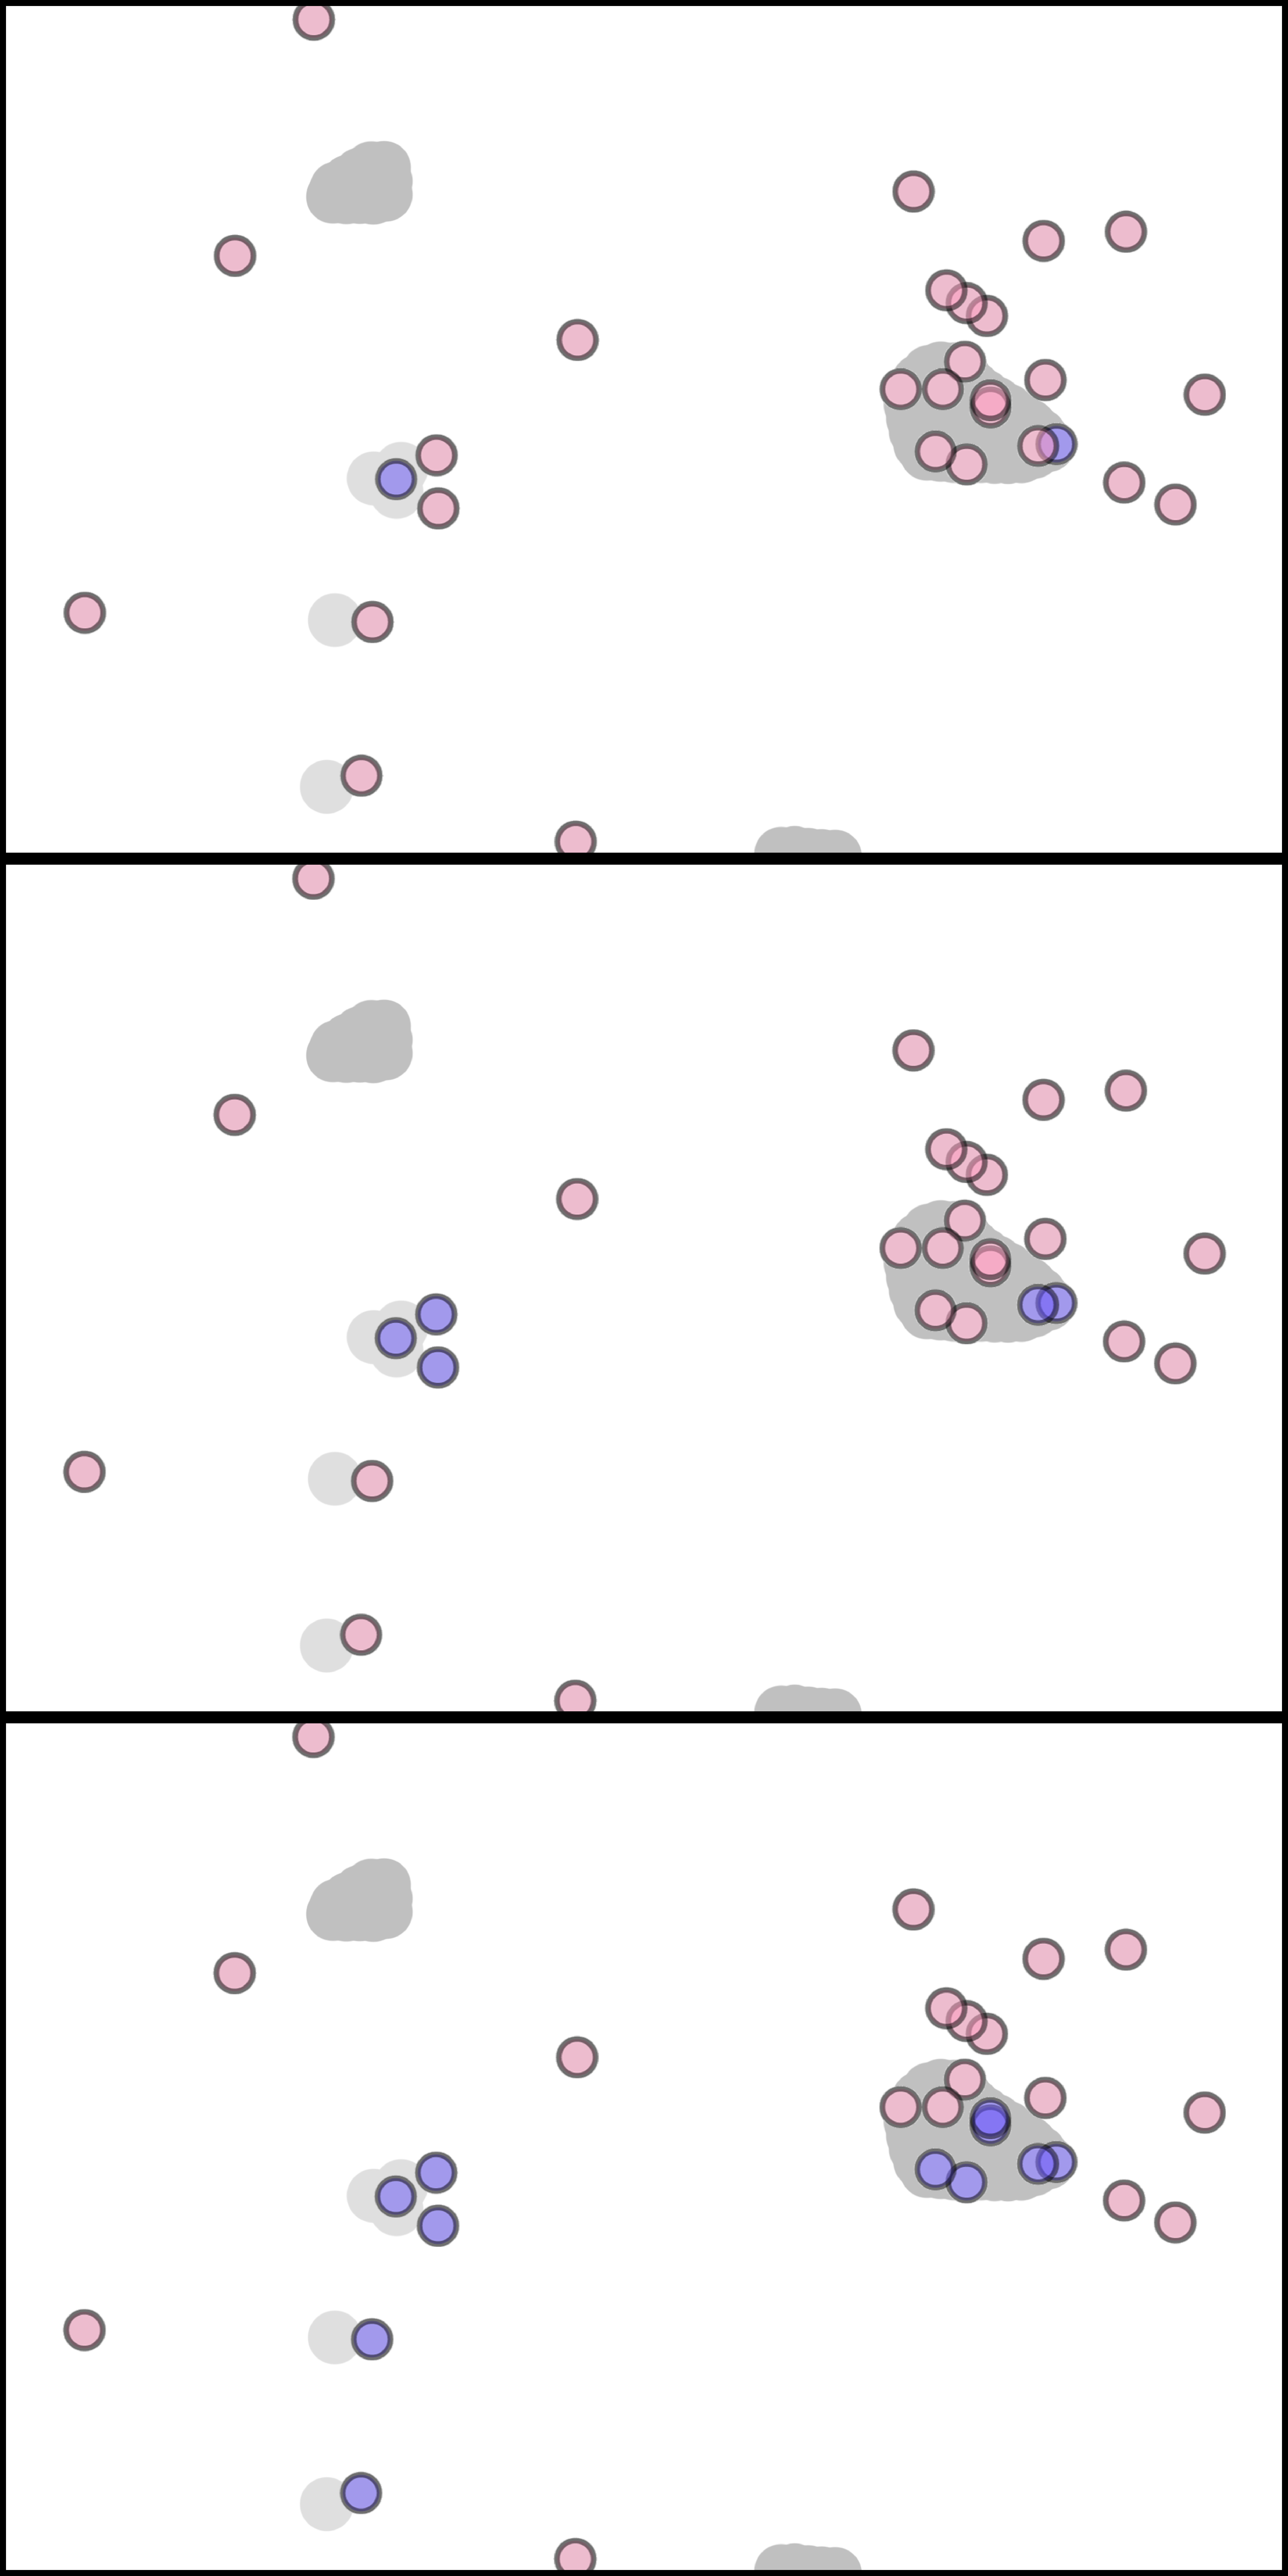
\includegraphics{figures/expansion-v} 

}

\caption{Example expansion over time from 2014 to 2016 (top to bottom) using fake data. Blue dots denote stores with Double Up, pink dots denote without. Gray sectors denote higher population density. The initial nodes can be seen in the top (2014) frame.}\label{fig:dufb-expansion}
\end{figure}

\subsection*{Selection of Control
Stores}\label{selection-of-control-stores}
\addcontentsline{toc}{subsection}{Selection of Control Stores}

Ideally, all remaining stores would have been available to use as a
control group but the company only approved that data be released for 15
stores. This left the added---and incredibly important---step of
selecting the control stores since the company approved, but did not
explicitly select, the 15 stores.

Selecting the control stores proceeded in two steps. First, stores that
either self-selected or were selected using some unobservable criteria
were matched using \emph{Coarsened Exact Matching} (CEM)
\citep{iacus_causal_2011}. Second, stores assigned Double Up were pooled
with nearby control stores and then scored using a linear probability
model. Each step is explained in detail.

\emph{Step 1: Coarsened Exact Matching}

The 6 stores classified as \texttt{self-selected} or \texttt{unobserved}
(stores \texttt{12} through \texttt{17}; see Table
\ref{tab:store-class}) were compared against all possible control stores
for matches. Matching was done across 5 dimensions: race, income,
population density, store attributes, store EBT sales. One variable per
dimension was selected: percentage of population that is
African-American (zip code level); people per square mile (zip code
level); median income for people who have received SNAP or similar
assistance (zip code level); the number of associates employed in each
store; and the percentage of total stores sales attributed to EBT/SNAP.

Of the 6 stores (stores \texttt{12} - \texttt{17}), only 3 produced
viable matches. However, each of the 3 matched stores had matched to
more than one control stores. The closest stores, by driving distance,
were selected as the tie-breaker for each matched store. Stores were
sufficiently far apart, with very sparsely populated areas between, that
``spill-over'' was considered unlikely. That is, it is considered
unlikely that a shopper near a store without Double Up would opt to
drive 30 or more minutes to shop at the store \emph{with} Double Up.

This left 12 stores to be allotted to the control group and 3 treatment
stores to be effectively discarded.

\emph{Step 2: Scoring via Linear Probability Model}

Assignment to treatment and control can be perfectly determined since we
know and observe the criteria used for assignment: geographic distance
from an initial store (node), SNAP EBT sales rank, and
demographics---specifically population density and percentage
African-American. A scoring function was created by fitting a linear
probability model to all stores within 140 kilometers of the two initial
pilot stores.

\[
\begin{aligned}
  \bm{s}  &= \widehat{P(\mathbf{D} = 1 | \bm{X}, \bm{N})} \\
          &= \mathbf{X} \bm{\hat \beta} + \hat \alpha \mathbf{N} + \left (\mathbf{X} \odot \mathbf{N} \right ) \bm{\hat \gamma}
\end{aligned}
\]

\(\bm{s}\) are the fitted values of the estimated linear probability
model; \(\mathbf{D} \in \{0,1 \}\) is a \(n \times 1\) vector of store
assignments to Double Up; \(\mathbf{X}\) is an \(n \times k\) matrix of
normalized observable covariates that determine assignment;
\(\mathbf{N} \in \{0, 1 \}\) is an \(n \times 1\) dummy vector denoting
the closest pilot store aka ``Node'', where \(0\) is \texttt{Node\ 0}
and \(1\) is \texttt{Node\ 1}. \(\odot\) represents element-wise
multiplication aka ``Hadamard product''.

Stores were sorted by the fitted values of the model, \(\bm{s}\). There
is perfect separation between Double Up stores and those without (see
Figure \ref{fig:score-plot}). Therefore, the top 11 stores by score
value are all Double Up stores. The next 12 stores by score value are
then allotted to the control group.

\begin{figure}
\centering
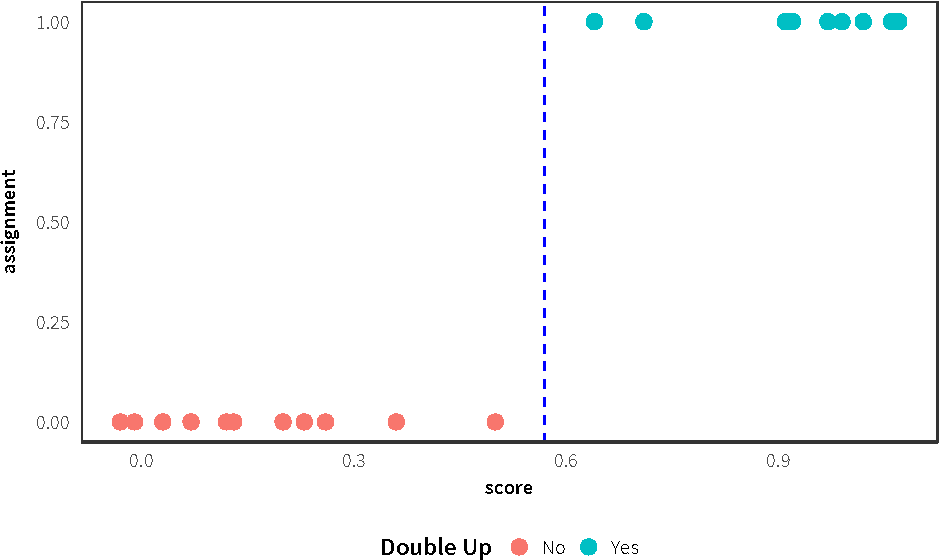
\includegraphics{noriega-prospectus-draft_files/figure-latex/score-plot-1.pdf}
\caption{\label{fig:score-plot}Store Score vs Double Up Assignment}
\end{figure}

\section*{Overview of Proposed Methods}\label{methods-1}
\addcontentsline{toc}{section}{Overview of Proposed Methods}

I will perform two separate analyses. This is a consequence of the store
selection issue outline in the data section. The main analysis will be
performed on the 9 \emph{assigned} stores and 12 \emph{control}
stores.\footnote{I'm excluding the 2 pilot store because they are never
  observed without DUFB.} In attempts to make use of as much data as
possible, I will also perform a smaller analysis with the 3
\emph{self-selected} stores matched using CEM. (Please see the
\protect\hypertarget{data-1}{}{Data} Section and Table
\ref{tab:store-class}) for more about \emph{assigned} and
\emph{self-selected} stores.)

Difference-in-Differences (DD) and Regression Discontinuity (RD) will
comprise the main analysis. DD will be the only method for the second
smaller analysis. I outline each analysis and its methods in the next
section.

The unit of analysis will be the store, not the individual; the data
cannot be linked to individuals. I assume the DUFB incentive, if
effective, will have a store-level effect. That is, if a store's
implementation of DUFB affects individual behavior, the effect should be
measurable after aggregating over all observed transactions. My proposed
analyses depend on this assumption but I am confident the effect will be
measurable.

I propose two outcome variables. The first is the proportion of SNAP EBT
dollars being spent or redeemed on fresh produce. If the incentive is
working, then I should see in increase in SNAP EBT dollars spending on
fresh produce. I'm certain this outcome variable will be available. I'm
not so certain about the second outcome variable, the total quantity of
fresh produce purchased. This depends on whether weight or quantity is
included in the data. This will depend on UPC matching. UPCs will be
possible, but matching to UPC databases is not always precise. Should
matching be poor, discerning what a product is, its weight, etcetera,
will be difficult, making the second outcome variable unreliable.

\textbf{Past Experience with Similar Data}

This is not my first experience working with transaction data. At this
point, I have more than 3 years working with transaction data.
Furthermore, this is not my first experience with transaction data where
(1) DUFB was implemented and (2) transactions were not linked to
individuals.

I performed an analysis in April of 2016 for FFN using 5 months of
transaction data from 3 small Detroit-area grocery stores. Figure
\ref{fig:trx-cycle} was produced with those data. It was easy to
distinguish when SNAP benefits were being used in those data. Likewise,
it was easy to tell when transaction made use of the DUFB incentive
(either an issuing of DUFB or a redemption). A simple aggregation could
determine the total amount of dollars spent per some unit time
(\emph{day} was the smallest possible unit of time). I expected data for
my prospectus will be very similar. The empirical models in the next
section were developed under these expectations of the data.

\subsection*{Difference-in-Differences}\label{difference-in-differences}
\addcontentsline{toc}{subsection}{Difference-in-Differences}

Difference-in-Differences (DD) models will be used in the main and
secondary analyses. The models will be identical but the data will
differ.

\textbf{The DD model 1 (DD1)}

The proposed model is as follows

\[
\begin{aligned}
  y_{ist}  &= \alpha_i + \beta_0 DUFB_{s} + \beta_1 POST_{t} + \delta (DUFB_{s} \cdot POST_{t}) + \sum_{j=1}^4 \theta_{j} I_{j}(t) + \epsilon_{ist}
\end{aligned}
\]

where \(y_{ist}\) is the outcome variable for store \(i\) in state \(s\)
during week \(t\). \(\alpha_i\) captures any time-invariant
store-specific effects. \(DUFB_{s}\) indicates whether store \(i\) has
or will be part of the DUFB incentive. \(POST_{t}\) indicates if week
\(t\) for store \(i\) lands in a post- or pre-DUFB year. Recall, there
are 3 years of data (2014 - 2016) and DUFB implementation is staggered
across stores. \(I_{j}(t)\) captures any cyclical effects due to the
monthly SNAP benefit transfer schedule. \(I_{j}(t) = 1\) if week \(t\)
is the \(j\)th week of the month, where \(j = 1,2,3,4\).

There are a total of \(156\) (\(52 \times 3\)) weeks in these data.
However, recall that the DUFB program is only live from August 1 to Dec
31 of each year. In other words, DUFB is being implemented for only
\(60\) of the \(156\) months. Things are further complicated by the way
the DUFB incentive worked between 2016 and years 2014 and 2015.

Time will be broken into weeks. The week of one year will be compared to
the same week in the following year. This is for three main reasons.
First, there is enough data per store to make precise estimates at the
weekly level. Given the small sample since (``small N''), expanding the
amount of observations along time (``bigger T'') will benefit the panel
models. Second, SNAP spending is cyclical, peeking in the 2nd week. This
is due to the state's monthly SNAP benefits transfer schedule. Benefits
are distributed every odd day of the month between the 3rd and 21st.
Each day maps to the digits \texttt{0} through \texttt{9}. SNAP
participants receive their benefits once a month on the day
corresponding to the last digit of their SNAP ID number. For example, ID
numbers that end in \texttt{0} receive their benefits on the 3rd of each
month. SNAP EBT benefits are spent quickly. As a result, there are
always fewer SNAP purchases during the 4th week of the month. And fewer
SNAP benefits means fewer transaction capable of receiving the DUFB
incentive. I believe it is better to capture this behavior in a model
versus smoothing it out by aggregating at the monthly level. Third, it
captures seasonal spikes that would also be smoothed out if aggregated
to the monthly level. I think it will be useful comparing, say, the the
week leading up the Thanksgiving between stores with and without DUFB.

The week-to-week cyclical pattern of SNAP EBT spending can be observed
in Figure \ref{fig:trx-cycle}. (Note that these are from a different
data source and different store chain, but from the same US state.) At
the start of the each month, SNAP EBT transactions (red line) increase
until peeking at the second week. The count then declines steadily
through the 4th week before once again spiking during the 1st week of
the following month. (Ignore the green line; these are DUFB counts from
a different data set.)

\begin{figure}

{\centering 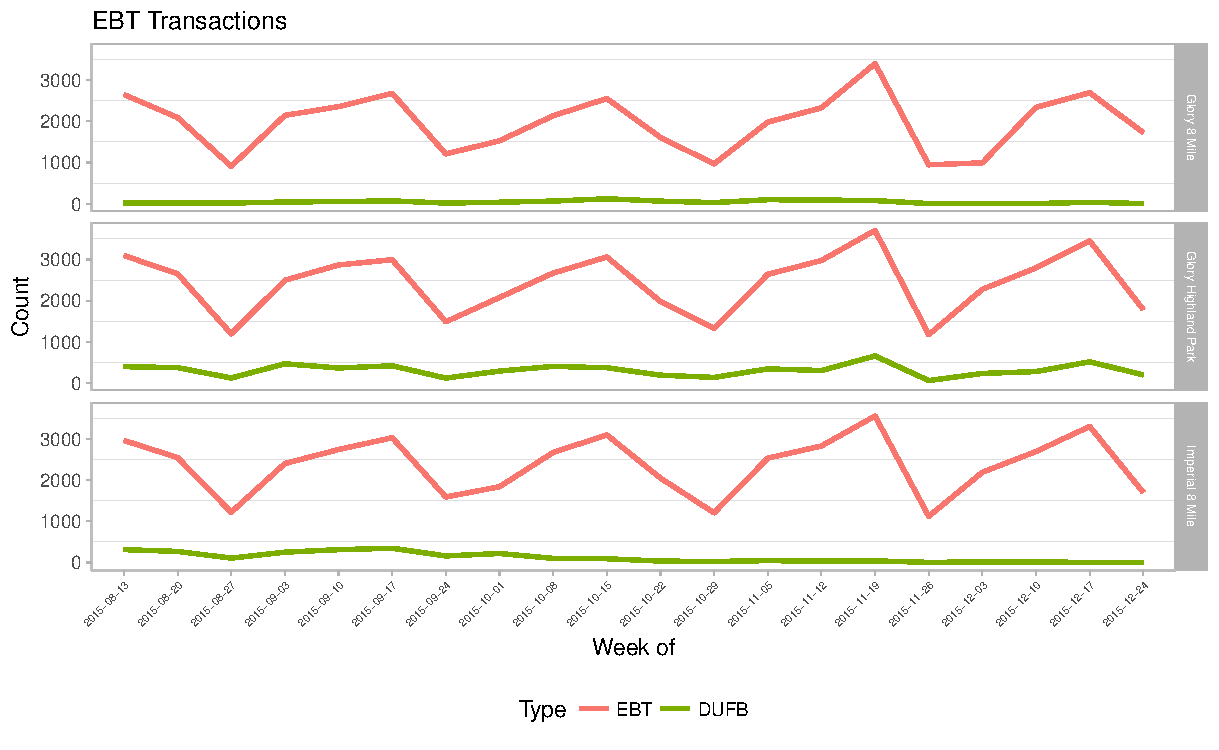
\includegraphics{figures/trx_counts} 

}

\caption{Example of how SNAP EBT benefits are spent in a predicable, week-to-week, cycle. It is the result of how benefits are distributed (uniformly across the first 3 weeks) and of how most SNAP participants spend their benefits (quickly and soon after being received). The red line is the count of transactions where SNAP EBT benefits were used as tender. Ignore the green line.}\label{fig:trx-cycle}
\end{figure}

Here is where I'm not sure what the best approach is.

Analysis of stores selected using \emph{known} and \emph{observable}
criteria.

\begin{enumerate}
\def\labelenumi{\arabic{enumi}.}
\tightlist
\item
  \textbf{Sample}: 11 Treated stores, 12 Control Stores across 3 years,

  \begin{enumerate}
  \def\labelenumii{\arabic{enumii}.}
  \setcounter{enumii}{2}
  \tightlist
  \item
    Within-group and between-group variation

    \begin{enumerate}
    \def\labelenumiii{\arabic{enumiii}.}
    \setcounter{enumiii}{3}
    \tightlist
    \item
      We lose some within-group variation as the 2 pilot stores are only
      ever observed as treated stores.
    \end{enumerate}
  \item
    Stores enter in waves. The staggering is used to produce extra
    variation between groups.
  \item
    T is 58 x 3 (weeks)

    \begin{enumerate}
    \def\labelenumiii{\arabic{enumiii}.}
    \setcounter{enumiii}{5}
    \tightlist
    \item
      Weeks is important because of MI SNAP schedule
    \item
      By the 4th week in every month, purchases with SNAP drop. It is
      important to capture this and not average it out by looking at
      monthly purchases.
    \end{enumerate}
  \item
    N is the same across time but the staggering shifts N for treated
    and control.

    \begin{enumerate}
    \def\labelenumiii{\arabic{enumiii}.}
    \setcounter{enumiii}{7}
    \tightlist
    \item
      \textbf{Table}: Create table showing the change in N subsample.
    \end{enumerate}
  \end{enumerate}
\item
  \textbf{Method 1}: Difference in Differences with FE

  \begin{enumerate}
  \def\labelenumii{\arabic{enumii}.}
  \setcounter{enumii}{4}
  \tightlist
  \item
    DinD seems appropriate.

    \begin{enumerate}
    \def\labelenumiii{\arabic{enumiii}.}
    \setcounter{enumiii}{5}
    \tightlist
    \item
      Larger and local economic forces should affect stores within each
      cluster equally.
    \end{enumerate}
  \item
    FE should remove any store-specific time-invariant attributes.
  \end{enumerate}
\item
  \textbf{Method 2}: Regression Discontinuity

  \begin{enumerate}
  \def\labelenumii{\arabic{enumii}.}
  \setcounter{enumii}{3}
  \tightlist
  \item
    \textbf{Fear 1:} using a running variable that is a function of
    other variables. Only seen one paper reference anything beyond one
    running variable \citep{papay_extending_2011}. Never seen a running
    variable that is score function.
  \item
    \textbf{Fear 2}: sample size here is small. RD performs better with
    large sample size.
  \end{enumerate}
\end{enumerate}

\subsection*{Difference-in-Differences with
Matching}\label{difference-in-differences-with-matching}
\addcontentsline{toc}{subsection}{Difference-in-Differences with
Matching}

Smaller analysis of the 3 stores that self-selected and were matched to
3 other stores.

\begin{enumerate}
\def\labelenumi{\arabic{enumi}.}
\setcounter{enumi}{2}
\tightlist
\item
  \textbf{Method:} Difference in difference been years 2015 and 2016

  \begin{enumerate}
  \def\labelenumii{\arabic{enumii}.}
  \setcounter{enumii}{2}
  \tightlist
  \item
    Power here will be small. Total N will be 6. Likely that nothing
    will be significant. But need to be transparent.
  \end{enumerate}
\end{enumerate}

\chapter{An Analysis of Non-recurrent TANF spending in Durham
County}\label{chapter-3}

\section*{Introduction}\label{intro-3}
\addcontentsline{toc}{section}{Introduction}

The Personal Responsibility and Work Opportunity Reconciliation Act of
1996 (aka ``welfare reform'') replaced the old welfare program, Aid to
Families with Dependent Children (AFDC), with Temporary Assistance for
Needy Families (TANF). TANF profoundly changed how states prioritize and
spend government welfare dollars. The result has been a gutting of
traditional cash assistance programs over the last 20 year. Cash
assistance used to accounted for 70\% of AFDC spending. Under TANF, cash
assistance accounts for 26\%, with ten states spending below 10\%
\citep{schott_how_2015}. Fewer and fewer dollars now reach families in
poverty with each passing year \citep{cbpp_chart_2016}.

The literature on the history and consequences of TANF over the past 20
years is vast.\footnote{\citet{ziliak_temporary_2015} provides a great
  overview on the history of TANF, including a great time line in the
  appendix. \citet{blank_what_2007} provides a great overview of what
  has been learned 20 years on.} However, for this paper, I will
spotlight the consequences of two welfare reform changes:

\begin{enumerate}
\def\labelenumi{\arabic{enumi}.}
\tightlist
\item
  The transfer of administrative authority to county and city
  governments.
\item
  The reporting requirement for basic assistance.
\end{enumerate}

The first change created opportunities for discrimination against
nonwhite welfare recipients. Caseworkers

\begin{itemize}
\tightlist
\item
  state and local governments attitudes about the poor and those most
  need of assistance. this can result in discriminatory distribution of
  benefits.

  \begin{itemize}
  \tightlist
  \item
    \citep{keiser_race_2004} investigate sanction rates for people
    receiving TANF benefits in Missouri. Sanctioning is decided by case
    workers at the local level. They find that nonwhites are sanction at
    higher rates compare than white TANF recipients in every local area.
  \end{itemize}
\end{itemize}

However, before doing so, it is important to understand how welfare was
financed under AFDC and how it changed under TANF.

\subsection*{Welfare Financing: AFDC vs
TANF}\label{welfare-financing-afdc-vs-tanf}
\addcontentsline{toc}{subsection}{Welfare Financing: AFDC vs TANF}

\textbf{Financing the AFDC Program}

The AFDC entitlement program was financed by a federal-state matching
grant system where the federal government shared the marginal cost of
every dollar spent on cash assistance by the states
\citep{ziliak_temporary_2015}. State spending on entitlements was
matched by the federal government at the Federal Medical Assistance
Percentage (FMAP), which ranged between 50\% and 83\%
\citep{falk_temporary_2016}. The FMAP matching rate was a function of a
state's economy. This assisted and encouraged poorer states to spend
money towards AFDC entitlements, even during an economic downturn.

The federal government, aside from helping fund AFDC, also determined
eligibility requirements. Even though the states did have the option to
extend some eligibility requirements, generally any impoverished mother
caring for a child was eligible to receive AFDC benefits. Benefits,
which came in the form of monthly cash assistance, had no work
requirement between 1935 and 1967. In 1967, a small work requirement was
added to received AFDC benefits, but beneficiaries were rarely sanction
for failing to meet the requirement. Federal requirements shifted with
passage of the Family Support Act of 1988 (FSA). FSA required mothers
with children over the age of 3 to participate in an education, work, or
training program to encourage a shift from welfare to work. States soon
began requesting waivers to try their own welfare-to-work programs in
place of AFDC \citep{blank_what_2007}. By 1996, waivers were approved
for 43 states. Welfare reform, which ended the AFDC program, occurred
soon after.

\textbf{Financing TANF}

TANF ended federal-state matching grant financing, replacing it with
federal fixed block-grant financing. Federal TANF spending for
block-grants is fixed at \$16.5 billion and has been since 1996.

Block-grant welfare financing profoundly changed how states prioritize
their spending. To receive a block-grant, states are required to spend
their own funds on programs supporting one of four TANF purposes:

\begin{quote}
C.F.R §§ 260.20 - What is the purpose of the TANF program?

The TANF program has the following four purposes:

\begin{enumerate}
\def\labelenumi{(\alph{enumi})}
\item
  Provide assistance to needy families so that children may be cared for
  in their own homes or in the homes of relatives;
\item
  End the dependence of needy parents on government benefits by
  promoting job preparation, work, and marriage;
\item
  Prevent and reduce the incidence of out-of-wedlock pregnancies and
  establish annual numerical goals for preventing and reducing the
  incidence of these pregnancies; and
\item
  Encourage the formation and maintenance of two-parent families.
\end{enumerate}
\end{quote}

The amount spent by each state must equal to 75\% of its FY1994
entitlement outlays. This is known as ``maintenance-of-effort'' (MOE)
spending.

Under the TANF block-grant financing, states have one true spending
incentive: to \emph{hit} the MOE level. Failure to meet the 75\% MOE
threshold results in an increases to 80\% the following year. States are
also penalized with a dollar-for-dollar reduction equal to the shortfall
between spending and the MOE threshold. However, unlike with AFDC, there
is no incentive in place to encourage states to spend their TANF
block-grants and no incentive to spend beyond. Under AFDC, every
additional dollar was matched by the federal government. That rate would
also increase if a state's economy hit a downturn. But under TANF, the
state pays the full marginal cost of every dollar spent \emph{beyond}
the TANF block-grant. Further discouraging spending is the fact that
states can roll-over any unspent TANF dollars to the following year,
without penalty.

However, it is not difficult for a state to hit its MOE. The flexibility
of the four TANF purposes, particularly the 3rd and 4th (c and d), means
practically any state spending is also MOE spending. There is also no
requirement for states to show how spending for a program satisfies one
of the four TANF purposes. The state need only outline how funds are
intended to be used and the purpose it falls under.

This is a much easier, more desirable way to spend funds compared to the
requirements when providing ``assistance''. ``Assistance'' is defined by
the US Department of Health and Human Services as any ongoing payment to
families to help meet basic needs \citep{falk_temporary_2016}. Any
spending that falls under this definition of assistance must be
reported, in detail, to the federal government. Detailed reporting of
who is receiving cash assistance, aka ``caseload'', is a bureaucratic
burden relative to the nonexistent reporting requirement for non-cash
assistance.

TANF is working as intended. TANF's block-grant financing, which
replaced AFDC's federal-state matching grant financing, was supposed to
provided greater spending flexibility and authority to the states.
Additionally, the reporting requirement ensure states were imposing TANF
work requirements and time limits for cash assistance. But it is
important to remember that welfare reform and TANF reflects the general
attitudes towards welfare in the late 1990s. There were too many people
were being rewarded for ``non-work'' and ``single parenthood''
\citep{rector_continuing_2003}. The reforms were needed to reduce
government dependency, child poverty, and illegitimacy, whilst also
encouraging work and strengthening two-parent families.

\textbf{TANF and Race}

This is coded language aimed against black

OVERVIEW

States determine how TANF monies are spent. Leads to heterogeneity in
how monies are spent. Most states have shifted monies to non basic
assistance. - why? - for all states, there is a disincentive to do so,
which is detailed reporting requirements if monies are given out as
basic assistance. - TANF money is flexible. possible to get block grant
and spend money on assistance that doesn't require large caseloads or
detailed reporting. - result? - without access to admin data, we know
little about where monies go - nonrecurring short-term, emergency
assistance falls under this area - the addition of work requirement
created a power dynamic between local gov and recipients - case workers
receive a lot of discretion about how funds are used and who got
sanction for failing to meet requirements - created a condition where
implicit racial biases and cultural narratives about who was more or
less deserving of welfare inevitably lead to nonwhites being sanctioned
more often, especially black women with children - true even when case
workers were also nonwhite - what i'm doing? - paper provides an
opportunity to verify observed discrimination in data that otherwise
goes unreported. - the data I have is short-term, emergency assistance
where people must apply in person. caseworkers have a lot of discretion
on who is approved or declined.

\begin{itemize}
\tightlist
\item
  TANF in NC

  \begin{itemize}
  \tightlist
  \item
    NC gets 302.2m with an MOE of 154.2m (75\%)

    \begin{itemize}
    \tightlist
    \item
      \citep{falk_temporary_2016}
    \end{itemize}
  \item
    where money is spent reflects state governments view on welfare and
    the poor
  \item
    Basic assistance is not a TANF priority for NC.

    \begin{itemize}
    \tightlist
    \item
      in FY2015, NC spent 9.2\% of TANF dollars on Basic Assistance
      (44th in the nation)
      \citep[\citet{schott_how_2015}]{us_dhhs_tanf_2015}\\
    \end{itemize}
  \item
    in recent past, has a rather restrictive approach to providing
    assistance
  \item
    imposed stronger work and saving requirements on beneficiaries in
    order to receive TANF dollars. reform occurred in 2013 known as
    ``Work First''

    \begin{itemize}
    \tightlist
    \item
      imposes requirements beyond those in AFDC
    \item
      families must sign a ``Mutual Responsibility Agreement''
    \item
      must work 20 hours a week
    \end{itemize}
  \item
    work requirements don't appear to pay off in the longterm when
    compared to intensive training and education programs
    \citep{pavetti_work_2016}
  \item
    access to cash assistance is affected by the overall conditions of
    how a state views welfare
  \item
    cultural narratives of dependency and ``undeserving poor'' lead to
    discrimination against minorities, especially of black women with
    children \citep{mannix_tanf_2013}
  \item
    implicit biases of caseworkers have been found to lead to lower
    average benefit payments and higher probability and severity of
    sanctions for black women with children versus white women
    \citep{soss_disciplining_2011}
  \end{itemize}
\end{itemize}

\subsection*{Nonrecurring Short-term
Benefits}\label{nonrecurring-short-term-benefits}
\addcontentsline{toc}{subsection}{Nonrecurring Short-term Benefits}

Non-recurrent short-term benefits\footnote{See
  \href{https://www.govregs.com/regulations/title45_chapterII_part260_subpartA_section260.31}{C.F.R.
  §§ 260.31.b}}:

\begin{enumerate}
\def\labelenumi{\arabic{enumi}.}
\tightlist
\item
  are designed to deal with a specific crisis situation or episode of
  need;\\
\item
  are not intended to meet recurrent or ongoing needs; and
\item
  will not extend beyond four months
\end{enumerate}

Non-recurrent short-term benefits do not count as basic assistance
(C.F.R. §§ 260.31.a). Therefore, these payments do not have to be
reported in detail to the federal government. However, these payments
\emph{do} count towards a state's MOE spending \citep{schott_how_2015}.

That said, non-recurrent short-term (emergency) benefits account for an
incredibly small amount of North Carolina's TANF and MOE spending. In
Fiscal Year 2015, North Carolina's combined TANF and MOE spending was
\$567,300,528 \citep{us_dhhs_tanf_2015-1}. Non-recurrent short-term
benefits accounted for \emph{0.9\%}---or \$4,919,303. Most of the
\$4,919,303---\$4,266,045 (86.7\%)---came from ``separate state
programs'' spending. This is spending that count towards state MOE but
are not funded by TANF.

\section*{Data}\label{data-3}
\addcontentsline{toc}{section}{Data}

The data are of nonrecurring short-term (emergency) benefits from the
Durham County Social Services in North Carolina.

\begin{itemize}
\tightlist
\item
  The type of services included can be found in the
  \href{http://dconc.gov/home/showdocument?id=7815}{Directory of
  Services} on DSS website.

  \begin{itemize}
  \tightlist
  \item
    financial assistance \citep[page
    11-14;][]{durham_county_department_of_social_services_directory_2016}.

    \begin{itemize}
    \tightlist
    \item
      DESCRIBE IN DETAIL
    \end{itemize}
  \end{itemize}
\end{itemize}

\subsection*{Preliminary Description}\label{preliminary-description}
\addcontentsline{toc}{subsection}{Preliminary Description}

\begin{itemize}
\tightlist
\item
  clean dataset contains 173654 records
\item
  includes data from 2011 to 2016 (by year of service)
\item
  DSS uses fiscal year. there are 5 complete fiscal years of data, 2012
  - 2016
\item
  in this subset, there are 93,409 unique records
\item
  there can be repeat
\end{itemize}

\bibliography{bib/book.bib}

\backmatter
\printindex

\end{document}
